\chapter{半導体の物理 ― スイッチの材料}
\label{chap2}

序章で見たとおり，電力変換の主役はエネルギーの流れ道を高速に切り替える半導体スイッチである。
本章では，そのスイッチの材料である半導体を物理から解き明かす。
半導体とは何か（\ref{sec2.1}節），ドーピング（\ref{sec2.2}節），キャリアの動き（\ref{sec2.3}節）と進み，
すべての素子の出発点であるpn接合（\ref{sec2.4}節）と金属との接合（\ref{sec2.5}節）を読み解く。

\begin{screen}
\noindent\textbf{この章の量が後で効く場所}\\[3pt]
\begin{箇条書}
\item バンドギャップ$E_g$ → 漏れ電流・高温動作・絶縁破壊電界（3章）
\item 移動度$\mu$とドーピング濃度 → オン抵抗（3章）・導通損失（5章）
\item 空乏層 → 耐圧・接合容量・スイッチング速度（3章）
\end{箇条書}
\end{screen}

%%======================================================================
\section{半導体とは何か ― キャリアの数を操れる物質}
\label{sec2.1}

物質は電気の流れやすさで大きく3つに分けられる。

\begin{箇条書}
\item \textbf{導体}\index{どうたい@導体}：電流が非常に流れやすい。銅，アルミニウム，金など
\item \textbf{絶縁体}\index{ぜつえんたい@絶縁体}：電流がほとんど流れない。ガラス，ゴム，酸化シリコンなど
\item \textbf{半導体}\index{はんどうたい@半導体}：両者の中間。シリコン，ゲルマニウム，炭化シリコンなど
\end{箇条書}

\textbf{半導体}の特長は，温度・不純物・電圧といった外部条件によって
\textbf{電流を流すか止めるかを外から制御できる}ことにある。
だから半導体はスイッチになれる。

電流$I$は単位時間に断面を通過する電荷$Q$の量（$I = dQ/dt$）であり，
電荷を運ぶ粒子を\index{きゃりあ@キャリア}\textbf{キャリア}という。
半導体のキャリアは電子（電荷$-e$）と，後で導入する正孔（電荷$+e$）である
（$e = 1.602\times10^{-19}$\,Cは\index{でんきそりょう@電気素量}電気素量）。
導体・半導体・絶縁体の違いは，\textbf{動けるキャリアがどれだけあるか}の違いである。

原子の中で電子は，とびとびの高さのエネルギーしか取れない。
原子が集まって固体になると，隣どうしの電子の軌道が重なり合って準位が多数に分裂し，
膨大な数の原子が集まるから，準位は事実上すき間なく並んで幅をもった帯になる。
これを\index{えねるぎーばんど@エネルギーバンド}\textbf{エネルギーバンド}という。

\begin{定義}[価電子帯・伝導帯・バンドギャップ]
\label{def2.1}
\begin{箇条書}
\item \index{かでんしたい@価電子帯}\textbf{価電子帯}：価電子が占めるバンド。低温では電子でほぼ満ちている
\item \index{でんどうたい@伝導帯}\textbf{伝導帯}：その上にある，電子が自由に動き回れるバンド
\item \index{ばんどぎゃっぷ@バンドギャップ}\textbf{バンドギャップ}$E_g$：両バンドの間の，電子が存在できないエネルギーの幅
\end{箇条書}
\end{定義}

満ちた価電子帯の電子は，満員電車の中の人と同じで，移動先の空きがないから動けない。
電流を運べるのは，伝導帯に上がった電子と，価電子帯にできた空席（正孔，後述）だけである。
物質の電気的性質は，このバンドの構造で決まる（\FIGref{fig2.1}）。

\begin{figure}[ht]
\begin{center}
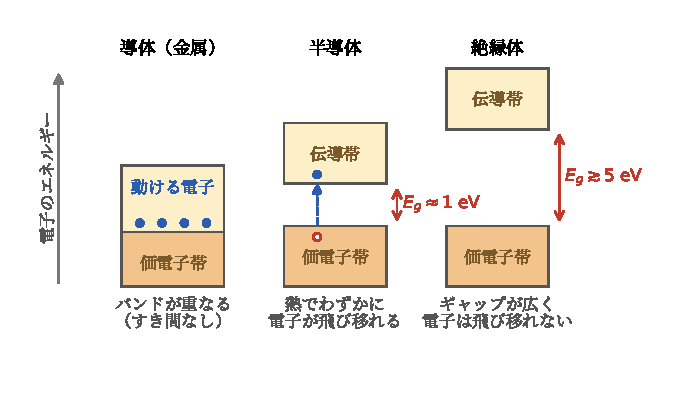
\includegraphics[clip]{figures/fig2.1.eps}
\end{center}
\caption{導体・半導体・絶縁体のバンド構造。バンドギャップの大きさが電気の流れやすさを決める}
\label{fig2.1}
\end{figure}

\textbf{導体}では価電子帯と伝導帯が重なるか，伝導帯に最初から電子があり，
動ける電子が常に多数ある。
\textbf{絶縁体}は$E_g$が大きく（5\,eV以上），室温の熱では電子が伝導帯に上がれない。
\textbf{半導体}は$E_g$が小さく（0.5〜3.5\,eV），室温でもわずかに電子が伝導帯へ上がり，
外部条件でその数を制御できる。
バンドギャップは，シリコン（Si）で約$1.1$\,eV，ゲルマニウム（Ge）で約$0.67$\,eV，
炭化シリコン（SiC）で約$3.3$\,eV，窒化ガリウム（GaN）で約$3.4$\,eVである。
eV（エレクトロンボルト）\index{えれくとろんぼると@エレクトロンボルト}は
電子1個が$1$\,Vの電位差で得るエネルギー（$1.602\times10^{-19}$\,J）である。
SiCとGaNは，シリコンの約3倍のバンドギャップをもつため
\index{わいどぎゃっぷはんどうたい@ワイドギャップ半導体}\textbf{ワイドギャップ半導体}と呼ばれる。
熱で伝導帯へ上がる電子の割合は$E_g$が大きいほど急激に減るから，
$E_g$が大きいほど漏れ電流が小さく高温に強く，後述の絶縁破壊電界も大きい。
この2つの利点が高耐圧・低損失のパワーデバイスに直結することを3章で見る。

バンド図には，「電子で満ちている高さの目安」として
\index{ふぇるみじゅんい@フェルミ準位}\textbf{フェルミ準位}$E_F$を書き込む。
$E_F$より十分低い準位はほぼ電子で満ち，十分高い準位はほぼ空である。
不純物を含まない半導体では，$E_F$はバンドギャップのほぼ中央にある。

熱で電子が価電子帯から伝導帯へ上がると，価電子帯に空席が1つ残る。
この空席を\index{せいこう@正孔}\textbf{正孔}という。
空席があれば隣の電子がそこへ移れ，移った跡にまた空席ができるから，
電子が次々に動く様子は\textbf{空席が逆向きに動く}様子として追う方が簡単である。
正孔は実在の粒子ではなく「電子の抜けた穴」に名前を付けたものだが，
電荷$+e$をもつ1つのキャリアとみなしてよいことが知られている。
以降は電子と正孔を対等な2種類のキャリアとして扱う。

%%======================================================================
\section{ドーピング ― n形とp形}
\label{sec2.2}

不純物を含まない純粋な半導体を
\index{しんせいはんどうたい@真性半導体}\textbf{真性半導体}といい，
電子と正孔が必ず対で生まれるから両者の濃度は等しい。
この濃度（\index{しんせいきゃりあのうど@真性キャリア濃度}\textbf{真性キャリア濃度}$n_i$）は
室温のシリコンで$1.5\times10^{10}\,\mathrm{cm^{-3}}$，
原子密度$5\times10^{22}\,\mathrm{cm^{-3}}$の1兆分の1にも満たず，
真性半導体はそのままではほとんど電流を流せない。

半導体に不純物をごく微量，意図的に混ぜることを
\index{どーぴんぐ@ドーピング}\textbf{ドーピング}という。
シリコン（Si）は\index{かでんし@価電子}\textbf{価電子}を4個もち，
結晶の中では各原子が隣の4個の原子と価電子を1個ずつ出し合って結び付いている。
ここに混ぜる不純物は2種類ある。

\begin{箇条書}
\item \index{どなー@ドナー}\textbf{ドナー}：電子を供給する5価の元素（リンP，ヒ素Asなど）
\item \index{あくせぷた@アクセプタ}\textbf{アクセプタ}：正孔を供給する3価の元素（ホウ素B，ガリウムGaなど）
\end{箇条書}

5価の元素をシリコン結晶に入れると，価電子5個のうち4個は周囲との結合に使われ，
1個が余る。余った電子はごく弱くしか束縛されず，室温の熱で簡単に伝導帯へ上がる。
バンド図では，ドナーは伝導帯のすぐ下の準位$E_d$から電子を供給する（\FIGref{fig2.2}(b)）。
こうして電子を多数もつ半導体を\index{えぬがたはんどうたい@n形半導体}\textbf{n形半導体}という。
逆に3価の元素を入れると，結合を4本作るには電子が1個足りない。
価電子帯の電子がこの不足分（アクセプタ準位$E_a$）に上がると，価電子帯に正孔が残る（\ref{fig2.2}(c)）。
正孔を多数もつ半導体を\index{ぴーがたはんどうたい@p形半導体}\textbf{p形半導体}という。

\begin{figure}[ht]
\begin{center}
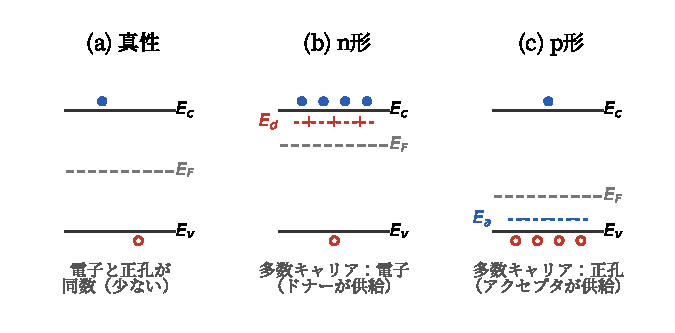
\includegraphics[clip]{figures/fig2.2.eps}
\end{center}
\caption{真性・n形・p形半導体のバンド図。ドーピングで多数キャリアとフェルミ準位が変わる}
\label{fig2.2}
\end{figure}

数が多い方のキャリアを\index{たすうきゃりあ@多数キャリア}\textbf{多数キャリア}，
少ない方を\index{しょうすうきゃりあ@少数キャリア}\textbf{少数キャリア}という。
n形では電子濃度$n$がほぼドナー濃度$N_d$に，p形では正孔濃度$p$がほぼアクセプタ濃度$N_a$に等しい。
フェルミ準位（電子で満ちている高さ）は多数キャリアの側，
つまりn形では伝導帯の近くへ，p形では価電子帯の近くへ寄る（\ref{fig2.2}）。

パワーデバイスでは，ドーピング濃度を$10^{13}$〜$10^{20}\,\mathrm{cm^{-3}}$の広い範囲で
場所ごとに作り分け，低濃度の層に高電圧を受け持たせ（耐圧），高濃度の層に電流を流す（低抵抗）。
この作り分けがデバイス設計そのものである（3章）。

\begin{screen}
\noindent\textbf{質量作用の法則}\\[3pt]
熱平衡にある半導体では，電子濃度$n$と正孔濃度$p$の積は
ドーピングによらず一定で，真性キャリア濃度$n_i$の2乗に等しい
（\index{しつりょうさようのほうそく@質量作用の法則}\textbf{質量作用の法則}）。
\begin{equation}
np = n_i^2
\label{eq2.1}
\end{equation}
多数キャリアを増やすと，少数キャリアはその分だけ減る。
\end{screen}

\begin{問}
\item p形シリコンにアクセプタを$N_a = 10^{17}\,\mathrm{cm^{-3}}$だけドーピングした。
多数キャリアと少数キャリアはそれぞれ何か。その濃度を求めよ（$n_i = 1.5\times10^{10}\,\mathrm{cm^{-3}}$）。
\end{問}

%%======================================================================
\section{キャリアの動き ― ドリフトと拡散}
\label{sec2.3}

キャリアが\textbf{動く}しくみは，ドリフトと拡散の2つしかない。

\begin{注意}
バンド図のエネルギー$E$と区別するため，本書では電場の大きさを$\mathcal{E}$と書く。
\end{注意}

半導体に電場$\mathcal{E}$をかけると，キャリアは電場から力を受けて加速されるが，
結晶中の原子や不純物に衝突しては向きを変えるため，平均すると一定の速度で流れる。
この流れを\index{どりふと@ドリフト}\textbf{ドリフト}，平均速度をドリフト速度$v_d$という。

\begin{screen}
\noindent\textbf{移動度と導電率}\\[3pt]
ドリフト速度は電場に比例し（$v_d = \mu\mathcal{E}$），
比例係数$\mu$を\index{いどうど@移動度}\textbf{移動度}という（単位はm$^2$/(V$\cdot$s)）。
電子濃度$n$，正孔濃度$p$の半導体のドリフト電流密度は
\begin{equation}
J = e (n \mu_n + p \mu_p) \mathcal{E} = \sigma \mathcal{E}
\label{eq2.2}
\end{equation}
と書ける（$\mu_n$，$\mu_p$は電子と正孔の移動度）。
$\sigma = e(n\mu_n + p\mu_p)$を\index{どうでんりつ@導電率}\textbf{導電率}という（単位はS/m）。
\end{screen}

式\ref{eq2.2}は「電流の流れやすさ＝キャリアの数$\times$動きやすさ」と読める。
室温のシリコンでは$\mu_n \approx 1350\,\mathrm{cm^2/(V\cdot s)}$，
$\mu_p \approx 480\,\mathrm{cm^2/(V\cdot s)}$であり，\textbf{電子は正孔の約3倍動きやすい}。
同じ抵抗なら電子で運ぶ方が少ないキャリアで済み，
これがパワーデバイスの主流がn形ベースの素子である理由の1つである（3章）。

\begin{例題}[ドリフト層の抵抗]
\label{rei2.1}
n形シリコン（$N_d = 10^{14}\,\mathrm{cm^{-3}}$，$\mu_n = 1350\,\mathrm{cm^2/(V\cdot s)}$）でできた
断面積$1\,\mathrm{cm^2}$，厚さ$100\,\mathrm{\mu m}$の層の抵抗を求めよ。
\begin{解答}
導電率は正孔の寄与を無視して
\begin{equation*}
\sigma = e N_d \mu_n = 1.602\times10^{-19} \times 10^{14} \times 1350
\approx 2.2\times10^{-2}\,\mathrm{S/cm}
\end{equation*}
厚さ$L = 100\,\mathrm{\mu m} = 10^{-2}$\,cm，断面積$A = 1\,\mathrm{cm^2}$だから
\begin{equation*}
R = \frac{L}{\sigma A} = \frac{10^{-2}}{2.2\times10^{-2} \times 1} \approx 0.45\,\mathrm{\Omega}
\end{equation*}
これはパワーMOSFETの内部で電圧を受け持つ層（ドリフト層）の抵抗の見積りそのものであり，
$10$\,Aを流せば$RI^2 = 45$\,Wもの損失を生む（オン抵抗の内訳は3章）。
\end{解答}
\end{例題}

キャリアの濃度に場所ごとの差があると，
キャリアは熱運動によって濃度の高い方から低い方へ広がる。
インクを水に垂らすと広がるのと同じ現象で，これを\index{かくさん@拡散}\textbf{拡散}という。
電場がなくても起こるこの流れが，次節のpn接合で空乏層を作る出発点になる。

\begin{問}
\item 上の囲みの$v_d = \mu\mathcal{E}$と式\ref{eq2.2}について，両辺の単位が一致することを確かめよ。
移動度の単位はm$^2$/(V$\cdot$s)，濃度の単位はm$^{-3}$とする。
\end{問}

%%======================================================================
\section{pn接合 ― 空乏層と整流作用}
\label{sec2.4}

\subsection{空乏層と内蔵電場}

p形半導体とn形半導体を1つの結晶の中で接合したものを
\index{ぴーえぬせつごう@pn接合}\textbf{pn接合}という。
ダイオードそのものであり，MOSFETもIGBTも内部はpn接合の組合せでできている。
接合面ではキャリアの濃度が急変しているから，拡散によって，
n形側の電子はp形側へ，p形側の正孔はn形側へ流れ込む。
流れ込んだ先は相手のキャリアだらけだから，
電子と正孔は出会って対で消滅する（\index{さいけつごう@再結合}\textbf{再結合}）。

再結合でキャリアが消えた接合面付近には，
n形側に電子を放出したドナーイオン（$+$），p形側に電子を受け取ったアクセプタイオン（$-$）が残る。
イオンは結晶に組み込まれていて動けない\textbf{固定電荷}である。
こうしてできた，動けるキャリアのほとんどない層を
\index{くうぼうそう@空乏層}\textbf{空乏層}という（\FIGref{fig2.3}(a)）。

\begin{figure}[ht]
\begin{center}
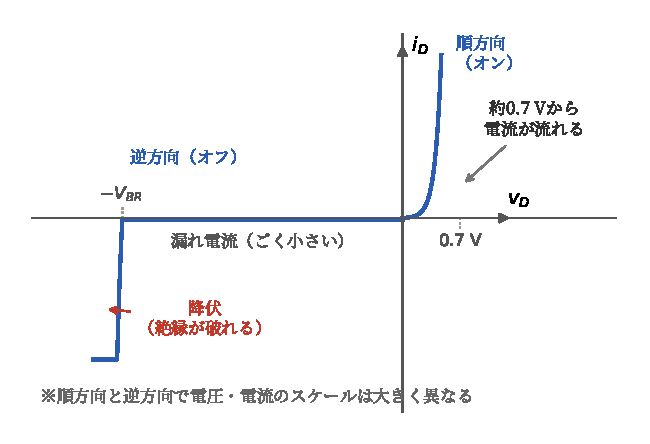
\includegraphics[clip]{figures/fig2.3.eps}
\end{center}
\caption{pn接合と空乏層。(a)拡散と再結合で固定イオンが露出し，(b)電荷密度$\rho(x)$が
(c)電場$\mathcal{E}(x)$を作り，(d)電位の差がバンドの曲がりとして現れる}
\label{fig2.3}
\end{figure}

空乏層には正負の固定電荷が向かい合って分布し（\ref{fig2.3}(b)），その間に電場ができる。
電場は正電荷（ドナーイオン）から負電荷（アクセプタイオン）へ，
つまり\textbf{n形からp形へ向かう}（\ref{fig2.3}(c)）。これを内蔵電場という。
内蔵電場は，電子をn形側へ，正孔をp形側へ押し戻す向き，
つまり\textbf{拡散をせき止める向き}に働く。
拡散が進むほど固定電荷が増えて電場が強まり，
やがて拡散と電場による引き戻し（ドリフト）がつり合って，正味の電流がゼロの平衡に落ち着く。

\subsection{バンドの曲がりと空乏層の幅}

電位は電場の向きと逆にたどると高くなるから，\textbf{n形側が高くp形側が低い}。
この電位差を\index{かくさんでんい@拡散電位}\textbf{拡散電位}（内蔵電位）$V_{bi}$という。
電子は負の電荷をもつから電位の高いn形側ほど電子のエネルギーは\textbf{低く}，
バンド図の縦軸は電子のエネルギーなので，バンドは電位の分布を上下反転した形に曲がる
（\ref{fig2.3}(d)の\textbf{バンドの曲がり}）。
曲がりの高さは$eV_{bi}$で，シリコンでは濃度によらずおおむね0.6〜0.8\,Vである。
なお，熱平衡ではフェルミ準位は全体で同じ高さにそろう（差があれば電流が流れてしまう）。

空乏層の幅について，押さえておくべきことは3つある。

\begin{箇条書}
\item \textbf{ドーピング濃度が低いほど空乏層は広い}。
同じ量の固定電荷を集めるのに，イオンの薄い領域では広い範囲が必要だからである。
\item 両側の濃度に差があるときは，\textbf{濃度の低い側に深く広がる}。
\item 空乏層は電圧を受け持つ層であり，\textbf{その中の電場には上限がある}
（\index{ぜつえんはかいでんかい@絶縁破壊電界}\textbf{絶縁破壊電界}，シリコンで約$3\times10^7$\,V/m）。
これを超えるとなだれのようにキャリアが増えて絶縁が破れる（降伏）。
\end{箇条書}

高い電圧に耐えるには，低濃度で広い空乏層を作って電場を薄く広く分担させるしかないが，
低濃度の層は例題\ref{rei2.1}で見たとおり抵抗が大きい。
\textbf{耐圧を取ればオン抵抗が増える} ―
このトレードオフがパワーデバイス設計の中心問題である（3章）。

\begin{問}
\item pn接合の両側でドーピング濃度が異なるとき，空乏層が濃度の低い側に深く広がるのはなぜか。
固定電荷のつり合いに注目して説明せよ。
\end{問}

\subsection{バイアスと整流性}

pn接合に外から電圧をかける（バイアスする）と何が起こるか（\FIGref{fig2.4}）。
p形側を正にする電圧（\index{じゅんばいあす@順バイアス}\textbf{順バイアス}）$V$をかけると，
内蔵電場が打ち消されて障壁は$e(V_{bi}-V)$に下がり，障壁を越えられるキャリアが急増して電流が流れる。
逆にp形側を負にする電圧（\index{ぎゃくばいあす@逆バイアス}\textbf{逆バイアス}）では
障壁が$e(V_{bi}+V)$に上がり，空乏層も広がって，電流はほとんど流れない。

\begin{figure}[ht]
\begin{center}
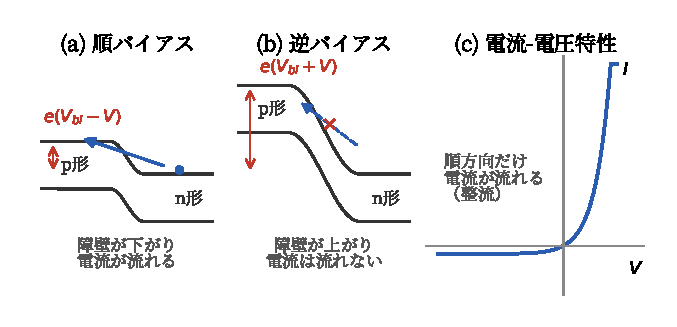
\includegraphics[clip]{figures/fig2.4.eps}
\end{center}
\caption{バイアスとpn接合の整流性。(a)順バイアスでは障壁が下がって電流が流れ，
(b)逆バイアスでは障壁が上がって止まる（左がp形側，右がn形側，青丸はn形側の電子）。
(c)一方向にだけ電流を流す}
\label{fig2.4}
\end{figure}

一方向にだけ電流を流すこの性質を\index{せいりゅうさよう@整流作用}\textbf{整流作用}という。
pn接合は，電圧の向きだけでオンとオフが決まる最も簡単なスイッチ ― ダイオードそのものである。
電流と電圧の関係式，および逆回復は3章で扱う。

%%======================================================================
\section{金属との接合 ― ショットキーとオーミック}
\label{sec2.5}

どんな半導体素子も最後は金属の電極につながるから，素子の中には必ず金属と半導体の接合面がある。
この接合は作り方しだいで2種類に分かれる。

\begin{箇条書}
\item \textbf{整流性接触}：一方向にしか電流を流さない（ショットキー接合）
\item \textbf{オーミック接触}：どちら向きにも低抵抗で電流を流す（電極に必要）
\end{箇条書}

どちらになるかを決めるのが\index{しごとかんすう@仕事関数}\textbf{仕事関数}，
すなわちフェルミ準位から電子1個を物質の外へ取り出すのに要するエネルギーである
（金属を$\phi_m$，半導体を$\phi_s$と書く。$\phi_s$はドーピングで変わる）。
仕事関数の異なる金属と半導体を接合すると，pn接合と同じ筋書きが始まる。
フェルミ準位の高い（仕事関数の小さい）側から低い側へ電子が移り，
界面に電荷がたまり，電場が生じ，半導体側のバンドが曲がる。
曲がりが両者のフェルミ準位の差をちょうど埋めたところで移動が止まる。
曲がるのはほとんど半導体側だけである（金属は電子密度がけた違いに大きい）。

n形半導体で$\phi_m > \phi_s$なら，電子は半導体から金属へ移り，
界面付近に電子のいない空乏層（ドナーイオンの正の固定電荷）ができて，
バンドが上に曲がり，電子の行く手をはばむエネルギー障壁ができる。
この障壁を\index{しょっときーしょうへき@ショットキー障壁}\textbf{ショットキー障壁}，
この接合を\index{しょっときーせつごう@ショットキー接合}\textbf{ショットキー接合}という。
pn接合と同様の整流性を示すが，順方向電圧が小さく（0.3〜0.4\,V），
少数キャリアを使わないため逆回復が速い（3章）。
$\phi_m < \phi_s$なら電子は金属から半導体へ移って界面の電子が増えるから障壁はできず，
どちら向きにも低抵抗で電流が流れる
\index{おーみっくせつごう@オーミック接合}\textbf{オーミック接合}になる。
p形半導体では結果が逆になる（\TABref{tab2.1}）。

\begin{table}[ht]
\begin{center}
\caption{金属と半導体の接合の型}
\label{tab2.1}
\begin{tabular}{c|c|c}
\hline
仕事関数の関係 & n形半導体 & p形半導体 \\
\hline
$\phi_m > \phi_s$ & 整流性（ショットキー） & オーミック \\
$\phi_m < \phi_s$ & オーミック & 整流性（ショットキー） \\
\hline
\end{tabular}
\end{center}
\end{table}

実際の素子の電極では，半導体の表面を高濃度（$10^{19}\,\mathrm{cm^{-3}}$以上）に
ドーピングする方法が広く使われる。
空乏層がきわめて薄くなって電子が障壁をすり抜けるため（トンネル効果），
仕事関数の関係によらずオーミック接合になる。

\begin{問}
\item 金（仕事関数$\phi_m = 5.1$\,eV）とn形シリコン（仕事関数$\phi_s = 4.3$\,eV）の接合は，
ショットキー接合とオーミック接合のどちらになるか。
\end{問}

%%======================================================================
\begin{章末問題}
\item \label{ex2.1}
室温のシリコン（原子密度$5\times10^{22}\,\mathrm{cm^{-3}}$，$n_i = 1.5\times10^{10}\,\mathrm{cm^{-3}}$）に
ドナーを$N_d = 10^{16}\,\mathrm{cm^{-3}}$だけドーピングした。
(a)不純物原子の割合，(b)電子濃度$n$と正孔濃度$p$を求めよ。

\item \label{ex2.2}
n形シリコンにドナーを$N_d = 10^{17}\,\mathrm{cm^{-3}}$だけドーピングした。
(a)電子濃度$n$と正孔濃度$p$，(b)導電率$\sigma$（正孔の寄与は無視してよい）を求めよ。
$n_i = 1.5\times10^{10}\,\mathrm{cm^{-3}}$，$\mu_n = 1350\,\mathrm{cm^2/(V\cdot s)}$とする。

\item \label{ex2.3}
pn接合に空乏層ができる過程を，拡散・再結合・固定電荷・内蔵電場の4つの語を使って説明せよ。

\item \label{ex2.4}
ワイドギャップ半導体（SiC，GaN）がパワーエレクトロニクスで注目される理由を，
(a)真性キャリア濃度，(b)絶縁破壊電界の2つの観点から説明せよ。
\end{章末問題}
